We begin our survey by showing some alarming Sybil attacks happening in the
real-world. Social network and micro-blogging websites are popular platforms for
organisations to improve public relations and their reputation, but they are
also platforms to spread propoganda. A recent article in the Atlantic described
how Twitter bots (Sybils) are shaping the 2016 US presidential
election\cite{atlantictwitterbots}. Over a third of pro-Trump tweets and almost
a fifth of pro-Clinton tweets, totalling at about 1 million, came from bots. The
article questions whether the bots are a threat to democracy because opinions of
real users are eclipsed by spam of bots.

\begin{figure}
  \centering
  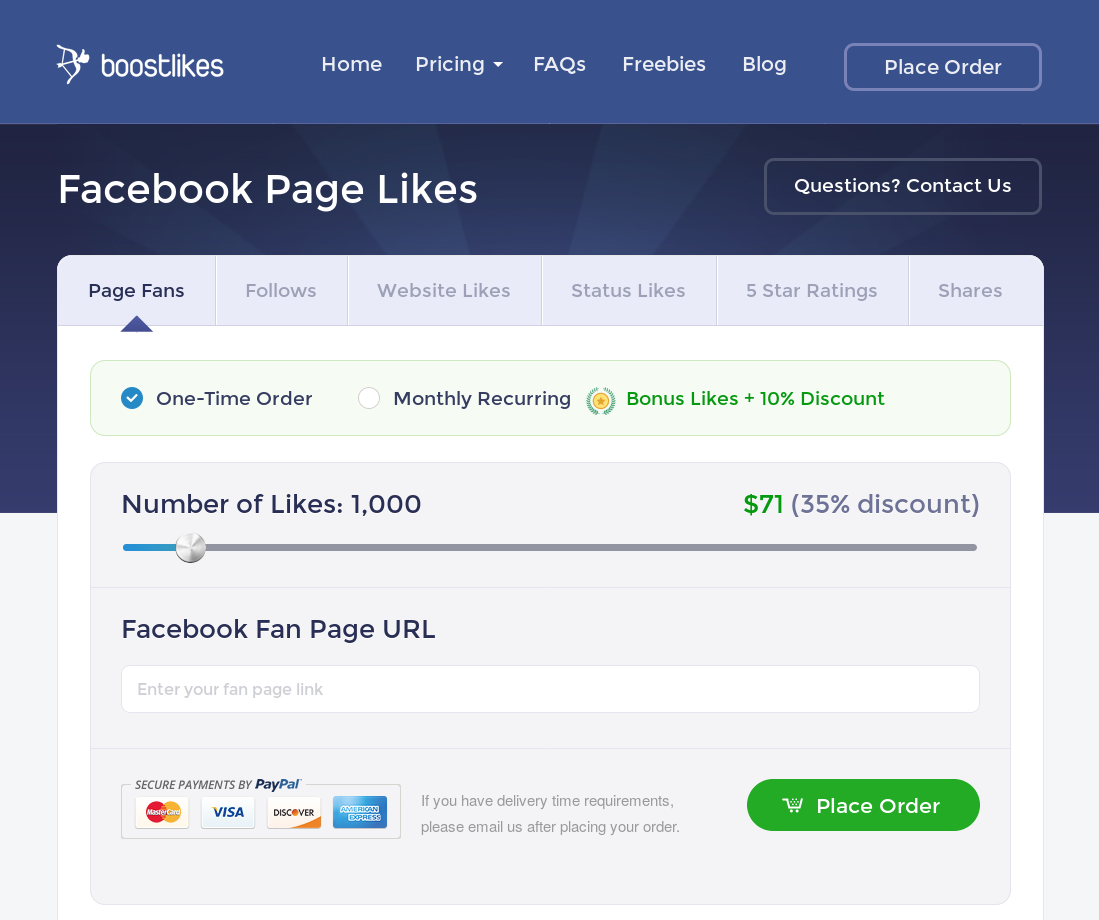
\includegraphics[width=0.5\textwidth]{boostlikes}
  \caption{Screenshot of the Facebook likes service page of boostlikes.com.}
  \label{fig:boostlikes}
\end{figure}

\begin{figure*}
  
\includegraphics[width=\textwidth]{socialformulae}
  \caption{Screenshot of the main banner on socialformulae.com.}
  \label{fig:socialformulae}
\end{figure*}

Using Sybils to manipulate public opinion is not only accessible to campaigners
with a large budget. There are marketplaces where anybody can purchase
reputation scores such as Twitter followers and Facebook likes. BoostLikes shown
on \autoref{fig:boostlikes} is a very professional looking website, it offers a
large range of services including Facebook likes, Twitter followers, Instagram
followers and YouTube views. SocialFormulae (\autoref{fig:socialformulae}) is a
similar service but at a much lower price point, one thousand Twitter followers
is only \$9.99.
% one thousand likes cost \$71 at the time of writing. 

Clearly, the defence mechanisms employed by social network and micro-blogging
websites are not adaquate to combat the Sybil attack. If the Sybils infiltrate
even more of our cyberspace, then it may become a form of censorship. In that
case, can we still be considered to have the right to freedom of speech?

%%% Local Variables:
%%% mode: latex
%%% TeX-master: "main"
%%% End:
